%=====================================================================
\section{Evaluation}\label{sec:evaluation}

\subsection{Questions}
\begin{description}
\item[RQ1] Is incremental admission equal to full recomputation, and do the secure checks return the plaintext findings?
\item[RQ2] On real policy changes, how large is the region of a change, and what would admission have held?
\item[RQ3] Which tools in the wild can be given a finite description of what they read?
\item[RQ4] How do admission and full recomputation scale with the number of rules and organisations?
\item[RQ5] What does admission across owners cost, compared with a full secure re-check and with an earlier sketch-based design?
\item[RQ6] How much do the findings themselves reveal under per-user and existence-only outputs?
\item[RQ7] Does federated learning improve the expected-use estimate that ranks held changes?
\end{description}

\subsection{Data and setup}\label{sec:setup}
\paragraph{AWS managed-policy history} The MAMIP repository records every version of the AWS managed IAM policies~\cite{mamip}. We replay its history from 3 November 2025, when it held \awsBasePol{} policies with \awsBaseSt{} statements, to 14 November 2026. A change event is a policy whose document differs from its previous version: \awsEvents{} events, of which \awsMod{} modify a policy and \awsAdd{} add one. Statements become rules over action vertices: action patterns are expanded against the \awsUniverse{} actions written explicitly in any version, so wildcard expansion is a lower bound, and resources and conditions are kept as canonical strings. Within a policy we report redundant pairs (same effect, action set and resources contained, conditions at least as strict) and allow/deny overlaps (shared actions, overlapping resource patterns), the latter an over-approximation on resources. For cross-policy findings we need two owners; we take the \awsAgentPol{} policies whose names identify an AI agent or assistant service (Bedrock, Amazon Q, the DevOps, security, FinOps and transform agents, and similar) as the authority of an agent, and the 11 AWS job-function policies as the authority of a person. An agent policy then amplifies a person by the actions it allows unconditionally on every resource that the job function does not allow at all, a lower bound on \Cref{def:cross} at action level. This pairing is constructed: AWS does not state that holders of a job function use these agents, and the name-based selection was not checked against service documentation.

\paragraph{Static real policies} The snapshot of 14 November 2026 holds 1,686 policies and 9,602 statements. 2,751 statements (28.7\%) are attribute sets as they stand, 2,534 (26.4\%) after expanding action patterns, and 2,790 (29.1\%) after reading equality conditions as attribute sets; 1,496 (15.6\%) carry conditions that are not sets, such as string patterns or null tests, and 31 (0.3\%) use negation. The model of Section~\ref{sec:model} therefore covers 8,054 statements (83.9\%). 4,288 statements (44.7\%) carry a condition and 87 (0.9\%) deny.

\paragraph{MCP tool schemas} The MCP Atlas Census contains \csTools{} tool records with input schemas from \csServers{} servers~\cite{mcpatlas2026}. We classify a tool as \emph{open-ended} when one of its string parameters carries code, SQL, a shell command, an expression or a URL chosen at call time, and as \emph{resource-addressed} when a parameter names a resource (identifier, path, table, bucket, repository and the like).

\paragraph{Constructed federations} No public data pairs the tool, data and usage policies of several organisations, so we generate them. Each of $K$ organisations owns 20 resources and hosts 10 tools; 10 further resources are co-owned by all. The population has 8 roles and 5 departments per organisation, $|S| = 40K$ user classes, plus one service account per organisation. Each organisation writes $n$ data rules and $n/2$ tool and usage rules; a rule constrains each subject attribute with probability 0.6 to one to three values, its key attribute to one to three owned or co-owned values, and is a permit with probability 0.8; 15\% of data rules grant service accounts. A tool reads one to three resources, each drawn from all resources of the federation with probability 0.4 and otherwise from those of its host, acts on behalf of the user with probability 0.6, and has one or two sinks. Events are drawn as 30\% data-rule, 15\% tool-rule and 8\% usage-rule insertions, 12\%, 6\% and 4\% deletions, 18\% redescriptions (half of which change only sinks or retention) and 7\% approvals. Decisions use deny-overrides. Unless stated, $K = 4$ and $n = 60$.

\paragraph{Earlier benchmarks} To compare with a sketch-based design for the same problem, we reuse its three benchmarks (Agentic, XS-ABAC and AMZ-Access; six domains, six collaboration scopes, 400 shared-scope rules per domain, five seeds), on which that design reported the false-positive rate of conflict detection and the cost of its decoder on secret shares.

\paragraph{Access logs} For RQ7 we use 32,769 real access requests of the Amazon employee access data~\cite{kaggle2013amazon}, with the eight largest business units as organisations that keep their logs private. The data have no timestamps, so past and future are a random 50/50 split per organisation; test negatives pair a user class with a resource drawn from the global popularity, so that popularity alone scores 0.5. We report AUROC over \rkSeeds{} seeds, overall and separately for resources the organisation has and has not seen.

\paragraph{Implementation} The analysis library, the secure protocol and all experiments are written in Python with NumPy; the code and the scripts that produce every number and figure are released with the paper. The secure protocol runs both servers in one process and counts every message in 4-byte field elements; it does not measure network latency and uses a non-cryptographic random generator, so it establishes correctness and communication, not deployed performance. Times are from a single process on a shared cloud virtual machine and are indicative.

\subsection{RQ1: exactness}\label{sec:exact}
On ten seeds of 300 random events each, the finding store after incremental admission equals a full recomputation after every one of the \eOneEvents{} events (\eOneMism{} mismatches). Every third event was also checked on secret shares: all \eOneSP{} same-layer checks (Algorithm~\ref{alg:pairsecure}, both directions) and all \eOneSC{} cross-layer cells with several owners (Algorithm~\ref{alg:ldsc}) returned exactly the plaintext findings. On the earlier benchmarks, the secret-shared pairwise checks returned the pooled oracle's conflicts, redundancies and gaps on all \exactRuns{} runs. Property tests compare the lemmas, the duality, attenuation and incremental maintenance with brute force on 3,000 random instances, and the coNP reduction on 2,000 random formulas. On the AWS history, no within-policy finding appeared or disappeared outside the changed statements in any of the \awsEvents{} events (\awsLocViol{} violations of \Cref{thm:locality}).

\subsection{RQ2: one year of real policy changes}\label{sec:aws}
\Cref{fig:aws} and \Cref{tab:aws} summarise the replay. Changes are frequent, about three a day, and they mostly grant: \awsGain{} events add actions, \awsMut{} of them state-changing ones, while only \awsLose{} remove any.

\begin{figure}[t]
\centering
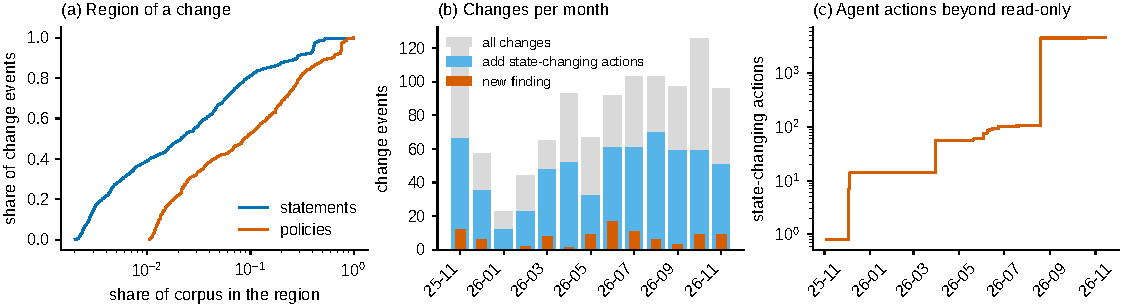
\includegraphics[width=\linewidth]{figures/fig_aws.pdf}
\caption{One year of AWS managed-policy changes replayed as events. (a) Distribution of the region of a change: share of all statements and of all policies that share an action vertex with a changed statement. (b) Changes per month, changes that add state-changing actions, and changes that introduce a finding. (c) Cumulative state-changing actions that agent-facing policies hold beyond the \texttt{ReadOnlyAccess} job function, counted at the change that introduced them.}\label{fig:aws}
\end{figure}

\begin{table}[t]
\centering\small
\caption{AWS managed-policy history, 3 November 2025 to 14 November 2026.}\label{tab:aws}
\begin{tabularx}{\linewidth}{Xr}
\toprule
Change events (modified / new policies) & \awsEvents{} (\awsMod{} / \awsAdd{})\\
Region, share of statements: median / mean / 90th percentile & \awsRegMed\% / \awsRegMean\% / \awsRegNinety\%\\
Events whose region holds under 1\% / under 5\% of statements & \awsRegUnderOne\% / \awsRegUnderFive\%\\
Region, share of policies: median / 90th percentile & \awsPolMed\% / \awsPolNinety\%\\
Findings changed outside the region & \awsLocViol\\
Events adding redundant pairs (pairs) & \awsRedEv{} (\awsRedPairs)\\
Events adding allow/deny overlaps (pairs) & \awsOvEv{} (\awsOvPairs)\\
Events on agent-facing policies / on job functions & \awsAgentEv{} / \awsJobEv\\
Agent events enlarging the amplification over some job function & \awsAmpEv\\
Agent events adding state-changing actions beyond \texttt{ReadOnlyAccess} (actions) & \awsAmpROEv{} (\awsAmpROAct)\\
Agent events adding state-changing actions beyond \texttt{ViewOnlyAccess} & \awsAmpVOEv\\
Events held by admission (any of the above findings) & \awsHeld{} (\awsHeldPct\%)\\
Admission time per event: median / 99th percentile & \awsIncMs~ms / \awsIncNinetyNine~ms\\
\bottomrule
\end{tabularx}
\end{table}

\paragraph{Locality} The region of a change is small for most changes: a median of \awsRegMed\% of statements and \awsPolMed\% of policies, and under 1\% of statements for \awsRegUnderOne\% of the events. The distribution has a long tail (\Cref{fig:aws}a): a change that writes a service-wide or global wildcard touches every statement on those actions, up to \awsRegMax\% of the corpus. Such changes are exactly the ones that deserve review, and their region is still computed from the index without reading the rest of the corpus.

\paragraph{What admission would have held} Admission would have held \awsHeld{} of the \awsEvents{} changes (\awsHeldPct\%). Inside policies, \awsRedEv{} changes introduced \awsRedPairs{} redundant statement pairs and \awsOvEv{} introduced allow/deny overlaps. Across our constructed pairing of agents and people, \awsAmpEv{} of the \awsAgentEv{} changes to agent-facing policies enlarged what an agent holds beyond some job function, and \awsAmpROEv{} of them gave the agent state-changing actions that a holder of \texttt{ReadOnlyAccess} does not have, \awsAmpROAct{} actions in total (\Cref{fig:aws}c). One change dominates: the modification of \texttt{\awsTopPol} on \awsTopDate{} added 12,202 actions, \awsTopAct{} of them state-changing and absent from \texttt{ReadOnlyAccess}. Whether this is intended is for the owners to decide; the point is that the change is visible at the moment it is made, with the affected job functions named. Changes to job-function policies, by contrast, almost never enlarged an amplification (one of \awsJobEv{} events), because they mostly add read actions.

\paragraph{Caveats} Allow/deny overlaps over-approximate resource overlap, so the \awsOvPairs{} overlap pairs are candidates; redundancy is exact for the syntactic containment we test. The amplification counts are lower bounds at action level for a pairing we constructed.

\subsection{RQ3: what tools let owners declare}\label{sec:census}
Of the \csTools{} tools, \csOpen{} (\csOpenPct\%) are open-ended: what they read is chosen at call time, so no finite $\reads(t)$ can be declared in advance, and \csSrvOpen{} servers (\csSrvOpenPct\%) expose at least one such tool. \csRes{} tools (\csResPct\%) name the resource they act on, so their reads can be declared at the granularity of a resource type. For open-ended tools the only sound description is everything the tool's identity may read; amplification is then computed on that over-approximation and blocked grants cannot be predicted. The classification is syntactic: a parameter named \texttt{url} that only selects a page of a known site is counted as open-ended, so the share is an upper estimate.

\subsection{RQ4: scaling}\label{sec:scale}
\Cref{tab:scale} and \Cref{fig:scaling} compare admission with full recomputation of all findings, over three seeds and 200 events per configuration. Full recomputation grows roughly with the square of the number of rules on each key vertex; admission grows with the rules on the event's key vertices only. At \scBigRules{} rules, recomputation takes \scBigFull~s and admission \scBigMed~ms in the median (\scBigPnn~ms at the 99th percentile), a ratio of \scBigSpeed{} on mean times, and the region holds \scBigReg\% of all slots in the median. With more organisations at fixed rules per organisation, the median admission time grows slowly, from 0.5 to 1.5~ms between 2 and 16 organisations, because each event touches the rules on a few key vertices; the 99th percentile grows faster, driven by events on co-owned resources, whose rules come from every organisation.

\begin{table}[t]
\centering\small
\caption{Admission against full recomputation on constructed federations (means over three seeds; 200 events each). Slots: rule pairs sharing a key vertex, cross-layer cells and usage cells. Speed-up: full time over mean admission time.}\label{tab:scale}
\resizebox{\linewidth}{!}{%
\begin{tabular}{rrrrrrrrr}
\toprule
$K$ & rules/org & rules & slots & full (s) & median (ms) & p99 (ms) & speed-up & region (\%)\\
\midrule
\csname @@input\endcsname generated/tab_scale 
\bottomrule
\end{tabular}}
\end{table}

\begin{figure}[t]
\centering
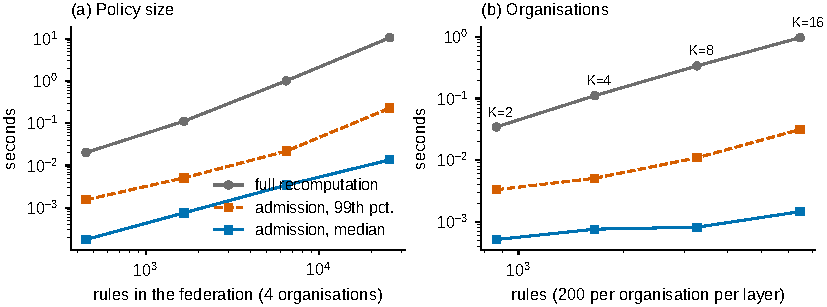
\includegraphics[width=0.98\linewidth]{figures/fig_scaling.pdf}
\caption{Time of full recomputation and of admission per event (median and 99th percentile), (a) as the number of rules grows with four organisations, (b) as the number of organisations grows with 200 rules per organisation per layer. Log--log scales.}\label{fig:scaling}
\end{figure}

\paragraph{What admission holds in the constructed federations} \Cref{tab:held} shows, per event type, the share of events that introduce each kind of finding. Redescriptions are held most often (89\%), mostly for usage violations and drift; tool-rule insertions for blocked grants and amplifications; data- and usage-rule insertions for conflicts with co-owners. Approvals never introduce a finding, since they can only remove drift. Overall \heldAll\% of events would be held. This rate reflects the random generator rather than practice, as the AWS history shows (\awsHeldPct\%); its role here is to exercise every branch of the admission check.

\begin{table}[t]
\centering\small
\caption{Share of events (\%) that introduce at least one finding of each type, by event type (ten seeds, \eOneEvents{} events).}\label{tab:held}
\resizebox{\linewidth}{!}{%
\begin{tabular}{lrrrrrrrr}
\toprule
Event & $n$ & Conf & Red & Gap & Amp & Viol & Drift & any\\
\midrule
\csname @@input\endcsname generated/tab_held 
\bottomrule
\end{tabular}}
\end{table}

\subsection{RQ5: cost across owners}\label{sec:costeval}
\Cref{tab:secure} reports the communication of admission on secret shares, against a secure re-check of the whole state. With four organisations and 1,643 rules, a full secure re-check exchanges \secMidFull~MB, while an event costs \secMidMed~kB in the median and \secMidMean~kB on average. With eight organisations and 3,237 rules, the full re-check costs \secBigFull~MB and an event \secBigMean~kB on average (\secBigPnf~kB at the 95th percentile); the tail comes from rule events on co-owned resources, whose cells involve every organisation. Most events need a single round of interaction in the median, because their only cross-owner work is one cell with one owner per side. On the AWS history, the flags-only amplification check of an agent or job-function change costs \awsSecKBMed~kB in the median under a comparable accounting (40 bytes per secure product: input sharing, Beaver opening and output), against \awsSecFullMBMed~MB for re-checking all actions; the largest change, which writes a near-global pattern, costs \awsSecMBMax~MB.

\begin{table}[t]
\centering\small
\caption{Communication of admission across owners on constructed federations (100 events each): full secure re-check of the state against one event. kB and MB of $10^3$ and $10^6$ bytes; ratio: full re-check over mean event.}\label{tab:secure}
\resizebox{\linewidth}{!}{%
\begin{tabular}{rrrrrrrrr}
\toprule
$K$ & rules & full (MB) & full rounds & median (kB) & mean (kB) & p95 (kB) & median rounds & ratio\\
\midrule
\csname @@input\endcsname generated/tab_secure 
\bottomrule
\end{tabular}}
\end{table}

\paragraph{Comparison with a sketch-based design} An alternative design summarises each domain's rules in hashed per-vertex counts and decodes anomalies from the sums of the other domains. Its decoder can also be run on secret shares. \Cref{tab:static} compares it with the exact checks of Algorithm~\ref{alg:pairsecure} on the same benchmarks, for a static analysis of all rules. The exact checks have no false alarms and cost less communication than the sketch at either size; the sketch with 512 bins falsely flags 12--55\% of non-conflicting rules, and with 4,096 bins its cost is about 30 times that of the exact checks. In its plain form, without secret sharing, the sketch also lets the other members of a scope reconstruct 66\% (512 bins) to 95\% (4,096 bins) of a domain's rules; the exact checks reveal only flags. Pooling all rules at a trusted auditor remains the cheapest exact option, at the price of disclosing every rule to it.

\begin{table}[t]
\centering\small
\caption{Static cross-domain analysis on three benchmarks (2,400 rules, six domains): sketch decoder on secret shares at 512 and 4,096 bins against the exact secret-shared checks. FPR: false-positive rate of conflict detection; MB: online communication between servers per domain (16 bytes per Beaver product); s: local computation per domain.}\label{tab:static}
\resizebox{\linewidth}{!}{%
\begin{tabular}{lrrrrrrr}
\toprule
& \multicolumn{2}{c}{Sketch, $B = 512$} & \multicolumn{2}{c}{Sketch, $B = 4096$} & \multicolumn{3}{c}{Exact (this work)}\\
\cmidrule(lr){2-3}\cmidrule(lr){4-5}\cmidrule(lr){6-8}
Benchmark & FPR & MB & FPR & MB & FPR & MB & s\\
\midrule
\csname @@input\endcsname generated/tab_static 
\bottomrule
\end{tabular}}
\end{table}

\subsection{RQ6: what the findings reveal}\label{sec:leakeval}
For each of the \leakRes{} resources of a constructed federation with \leakClasses{} user classes, we measure the events a tool host needs to learn the owner's decision row on that resource. With per-user outputs one event suffices, as Proposition~\ref{prop:probe}(i) states. With existence-only outputs and adaptive group testing by binary splitting, the host needs on average \leakProbes{} events, against an information-theoretic minimum of about \leakEntropy{} bits per row; rows are dense here (on average \leakDenied{} of \leakClasses{} classes denied), which makes splitting less efficient than asking class by class. A quota of $Q$ events per period therefore bounds the leakage to $Q$ bits, and owners that need per-user findings accept that a partner learns which of its users are refused.

\subsection{RQ7: ranking by expected use}\label{sec:rankeval}
\Cref{tab:rank} and \Cref{fig:rank} report the expected-use estimate behind \eqref{eq:impact}. The federated hyperedge model reaches AUROC \rkFed, against \rkCount{} for the best local method, simple exercise counts, so the overall gain is small. The gain is concentrated where federation can help: on resources new to the organisation, local methods are at chance (0.500), while the federated model reaches \rkFedNew. On resources the organisation already knows, federation adds nothing (\rkFedSeen{} against the same model's local 0.727). The federated model stays 0.07 below pooling all logs (\rkPool), and the propagation step does not help (\rkProp{} federated). We therefore use the model only to order held changes, and only claim benefit for tools and resources that are new to an organisation.

\begin{table}[t]
\centering\small
\caption{Expected-use estimation on real access requests (AUROC; mean over organisations and \rkSeeds{} seeds; ``new'': resources absent from the organisation's past log). Pooled: all logs at one place, an upper bound that discloses them.}\label{tab:rank}
\resizebox{\linewidth}{!}{%
\begin{tabular}{lrrrrrr}
\toprule
& \multicolumn{2}{c}{Local} & \multicolumn{2}{c}{Federated} & \multicolumn{2}{c}{Pooled}\\
\cmidrule(lr){2-3}\cmidrule(lr){4-5}\cmidrule(lr){6-7}
Model & all & new & all & new & all & new\\
\midrule
\csname @@input\endcsname generated/tab_rank 
\bottomrule
\end{tabular}}
\end{table}

\begin{figure}[t]
\centering
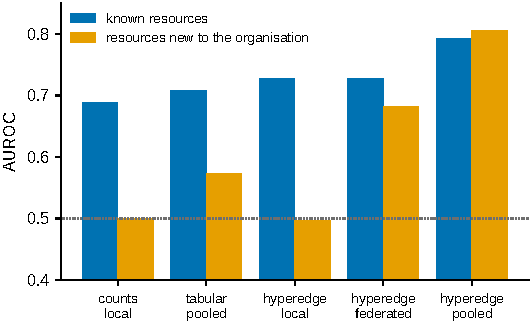
\includegraphics[width=0.62\linewidth]{figures/fig_rank.pdf}
\caption{AUROC of expected-use estimation on known resources and on resources new to the organisation.}\label{fig:rank}
\end{figure}
